%!TEX root = ../document.tex
\chapter{SQL-Injection}
Eine SQL-Injection ist ein Angriff auf eine Benutzerschnittstelle, die mit einer Datenbank im Hintergrund kommuniziert. Dabei werden SQL-Befehle z.B. über die normalen Eingabefelder einer (Web-)Applikation an die Datenbank geschickt und dort ausgeführt. Dies kann dazu führen, dass der Angreifer Zugriff auf sensible Daten oder Anwendungen erhält oder sogar die komplette Datenbank löschen kann. 

\section{Erklärung}
Beinahe jede moderne Anwendung - sei es eine Webanwendungen wie Facebook oder eine klassische Client-Server-Applikation mit einer speziellen Benutzeroberfläche wie SAP ERP - verwendet im Hintergrund ein Datenbankmanagementsystem zur Verwaltung und Speicherung der Applikationsdaten. Die Datenbank ist dabei i.d.R. von größerem Wert als die Anwendung selbst. In Industrieunternehmen enthalten Datenbanken z.B. Informationen zu Mitarbeitern, Kunden, Finanztransaktionen, Produktionsplänen oder geheime Dokumente der Produktentwicklung. Datenbanken sind somit ein kritischer Bestandteil vieler Unternehmen. Deren Verfügbarkeit und Sicherheit ist wichtig für den Fortbestand des Unternehmens und daher auch gesetzlich geregelt\footnote{Siehe \url{https://www.bsi.bund.de/DE/Themen/ITGrundschutz/ITGrundschutzKataloge/Inhalt/_content/baust/b05/b05007.html} }.

Kriminell motivierte Hacker haben daher ein hohes Interesse daran, Zugang zu diesen Daten zu erhalten. Eine möglicher Zugriffsweg hierfür ist das Ausnutzen von Schwachstellen durch SQL-Injections.

Um SQL-Injections durchführen zu können, wird lediglich ein grundlegendes Verständnis klassischer Anwendungsarchitekturen und der Datenbankabfragesprache SQL benötigt. Die Grundlagen hierzu werden nachfolgend erläutert.

\subsection{Grundlagen Datenbanksysteme}
\emph{Datenbanksysteme} (DBS) sind ein weithin genutztes Hilfsmittel zur rechnergestützten Organisation, Erzeugung, Veränderung und Verwaltung großer Datensammlungen und stellen in vielen Unternehmen und Organisationen die zentrale Informationsbasis zu ihrer Aufgabenerfüllung bereit. Ein DBS besteht aus einem \emph{Datenbankmanagementsystem} (DBMS) und einer oder mehrerer Datenbanken. Eine Datenbank ist eine Zusammenstellung von Daten samt ihrer Beschreibung (Metadaten), die persistent im DBS abgelegt werden.

Das DBMS bildet die Schnittstelle zwischen den Datenbanken und dient den Benutzern zur Datenverwaltung und -Veränderung. Die zentralen Aufgaben eines DBMS sind im Wesentlichen die Bereitstellung verschiedener Sichten auf die Daten (Views), die Konsistenzprüfung der Daten (Integritätssicherung), die Autorisationsprüfung, die Behandlung gleichzeitiger Zugriffe verschiedener Benutzer (Synchronisation) und das Bereitstellen einer Datensicherungsmöglichkeit, um im Falle eines Systemausfalls zeitnah Daten wiederherstellen zu können.

Der Zugriff auf die Daten erfolgt mithilfe einer standardisierten Abfragesprache, der \emph{Structured Query Language} (SQL). Durch sie können Datenstrukturen angelegt und verändert werden, neue Daten zur Datenbank hinzugefügt sowie bestehende Daten verändert oder gelöscht werden. 

\subsection{3-Schichten-Architektur}
\begin{figure}[H]
	\centering
	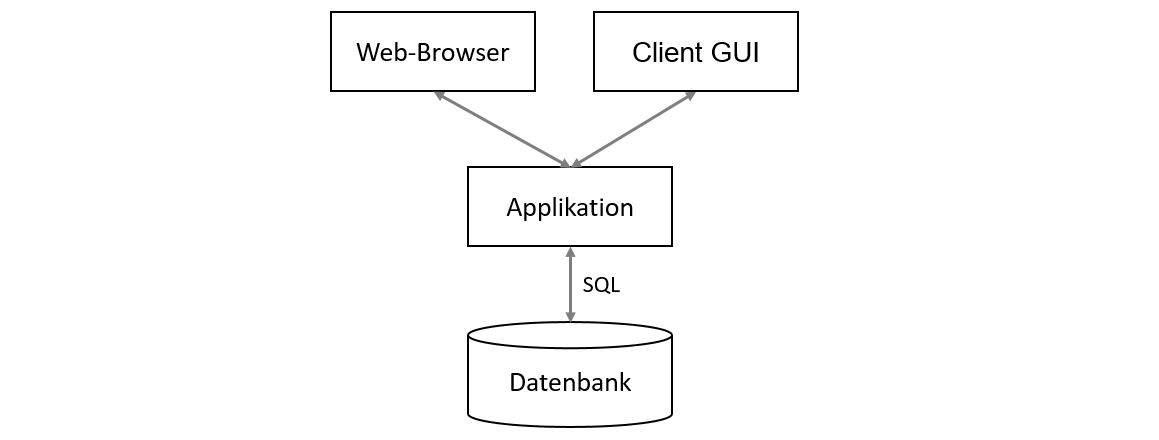
\includegraphics[width=\textwidth]{images/SQL_Injection/3TierArchitecture.jpg}
	\caption{3-Schichten-Architektur}
	\label{fig:3TierArchitecture}
\end{figure}

DBS werden von Endanwendern nicht direkt genutzt, sondern werden durch die Applikation und graphische Oberflächen verschalt. Der Benutzer greift z.B. via HTTP über die Oberfläche auf die Applikation zu. Die Applikation selbst ist mit einem dedizierten Datenbankbenutzer mit dem DBS verbunden, die Kommunikation erfolgt über SQL. Diese Architektur wird wegen ihrer drei Ebenen - der Präsentations-, der Logik- und der Persistenzschicht - auch als 3-Schichten-Architektur bezeichnet (vergleiche Abbildung \ref{fig:3TierArchitecture}). 

Die Applikationen stellen dem Benutzer Eingabefelder zur Verfügung, mittels derer die Benutzer Daten auslesen, verändern oder neu erzeugen können. Die Benutzereingaben werden zu bereits vorgefertigten SQL-Statements hinzugefügt und an das DBS gesendet. Das DBS verarbeitet das Statement und sendet eine Antwort an die Anwendung zurück.

\subsection{Der Angriff}
Bei einer SQL-Injection werden, wie der Name schon impliziert, (Teile von) SQL-Statements an die normalen Benutzereingaben angehängt, um somit die Logik und die Sicherheitsmechanismen der Applikation zu umgehen.

Der SQL-Interpreter des DBMS führt das ursprüngliche und die angehängten Statements aus. Mittels geschickter SQL-Injections können über harmlose Benutzerschnittstellen ganze Datenbanken gelöscht werden.

\section{Vorbereitung}
Für die Ausführung des Tutorials wird Kali Linux 2.0 mit eingerichteter Security Workbench benötigt. Alternativ kann das Skript auf einem anderen beliebigen Linux-System verwendet werden, in dem MySQL und Apache2 installiert sind. Zur korrekten Initialisierung der Webanwendung muss ggf. der Pfad zum Apache-Webserver in der Datei 'initializeDB.py' geändert werden. Die zu konfigurierenden Pfade im Quellcode sind entsprechend gekennzeichnet.

\section{Ablauf}
\subsection{Aufbau des Login-Web-Services}
Das Tutorial wird über die Security Workbench unter dem Hauptmenüpunkt 4 aufgerufen. Zu Beginn wird der Apache2-Webserver und das MySQL-DBMS gestartet. Anschließend wird die Datenbank initialisiert. Dabei wird folgendes Schema erstellt:
\begin{figure}[H]
	\centering
	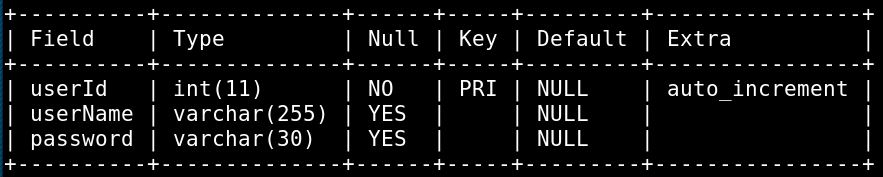
\includegraphics[width=\textwidth]{images/SQL_Injection/table_secretUserData.jpg}
	\caption{Tabellenstruktur der Tabelle \enquote{secretUserData}}
	\label{fig:table_secretUserData}
\end{figure}

Nun stehen verschiedene Tutorials zur Verfügung. Sie alle basieren auf demselben Web-Service, einem Login für eine Website (siehe Abbildung \ref{fig:user}). Der Web-Service wurde in HTML/CSS, JavaScript und PHP entwickelt. Die Benutzereingaben werden auf der HTML-Seite entgegen genommen und über einen Ajax-Aufruf an PHP übergeben. 

\begin{figure}[H]
	\centering
	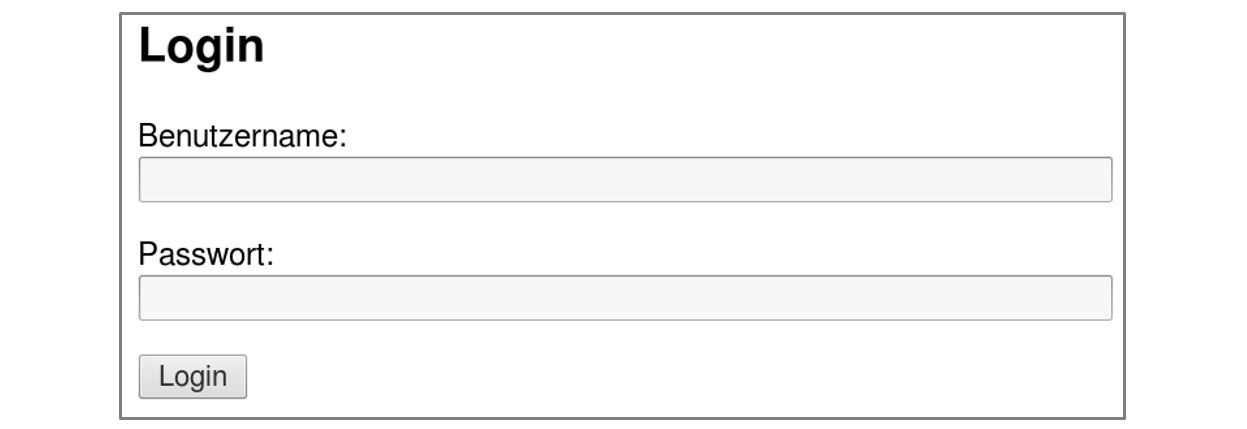
\includegraphics[width=\textwidth]{images/SQL_Injection/login.jpg}
	\caption{Login-Oberfläche des Web-Services}
	\label{fig:user}
\end{figure}

Dort werden die Benutzereingaben in ein vordefiniertes SQL-Statement eingefügt (siehe Listing \ref{lstlisting:SQL-Statement}) und an das DBS zur Ausführung übermittelt. Die Antwort des Servers, ein oder mehrere zutreffende Tupel mit der User-ID, dem User-Namen und dem User-Passwort werden anschließend unterhalb des Eingabefelds in dem Web-Service angezeigt. Dort ist ebenfalls das im DBS ausgeführte SQL-Statement zu sehen.

\begin{lstlisting}[caption=SQL-Statement\label{lstlisting:SQL-Statement}]{Name}
$query = '
	SELECT * 
	FROM secretUserData 
	WHERE userName = "'.$username.'" 
	AND   password = "'.$password.'";
';
\end{lstlisting}

Zudem sind zwei Buttons verfügbar, mit denen die Tabellenstruktur sowie der momentane Inhalt der Tabelle angezeigt werden können.

\subsection{SQL-Injection zum Auslesen von Daten}
Im ersten Teil des Tutorials werden mittels einer einfachen SQL-Injection Daten aus der Datenbank gelesen, auf die man über die Anwendung eigentlich keinen Zugriff hätte. Über die zwei Eingabefelder \enquote{Benutzername} und \enquote{Login} kann sich der Benutzer bei einer Anwendung anmelden. Die Eingaben werden an die Datenbank geschickt und in einem SELECT-Statement überprüft. Anschließend wird der selektierte Datensatz zurück geschickt.

Als erstes melden wir uns mit einem schon bekannten User und Passwort an, um die Funktionsweise zu testen. Nutze hierzu den User \colorbox{altgray}{\lstinline|Douglas Adams|} mit dem Passwort \colorbox{altgray}{\lstinline|DontPanic!|} und drücke auf den "Login"-Button."

\begin{figure}[H]
	\centering
	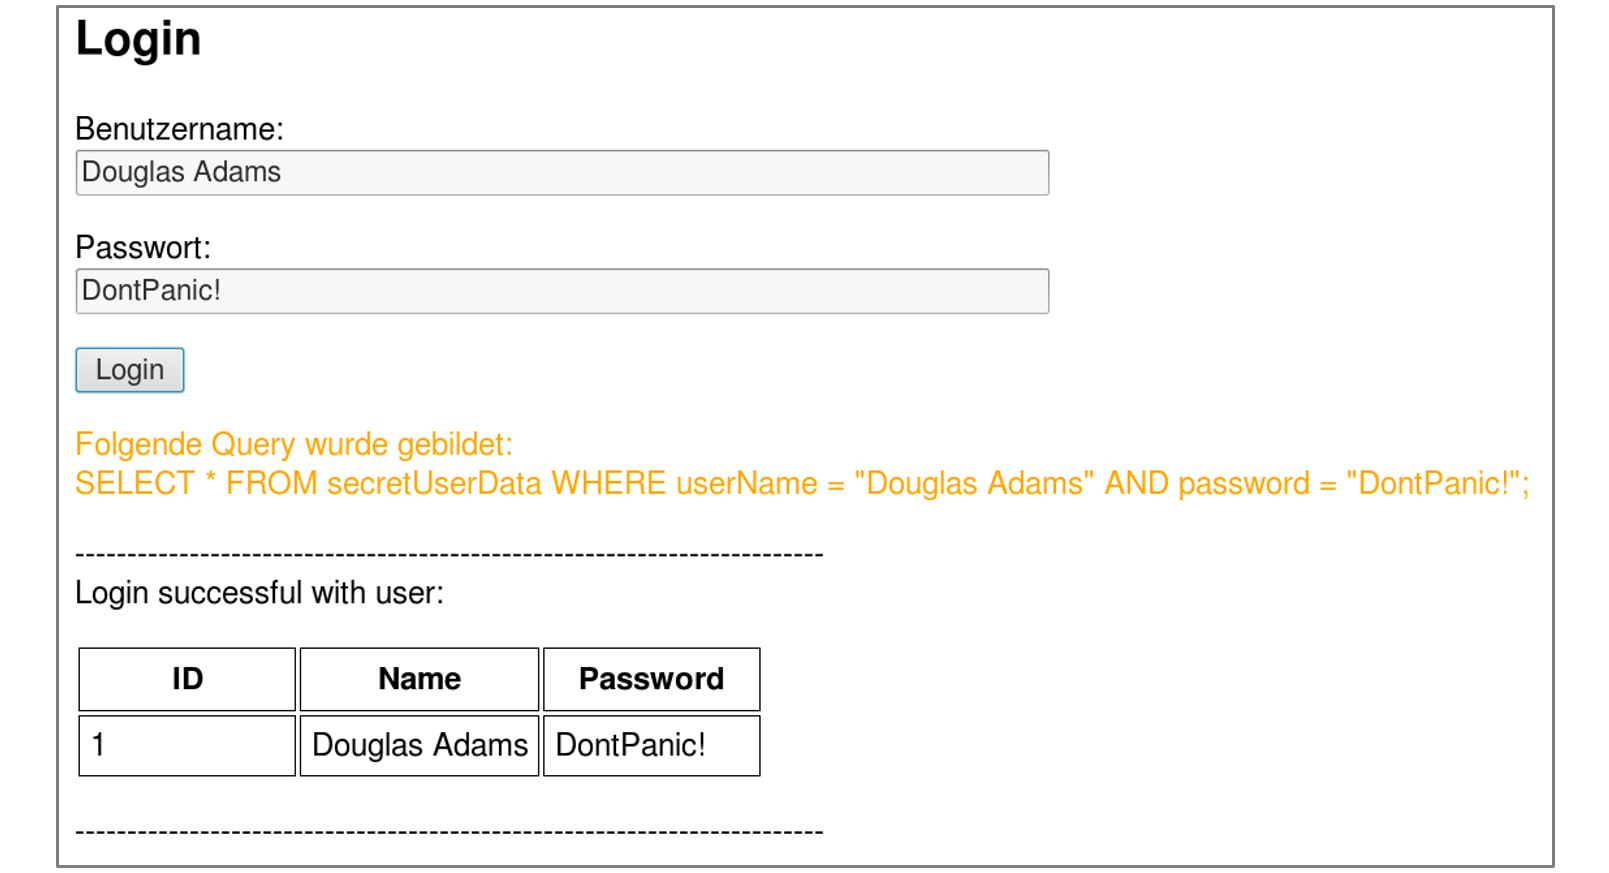
\includegraphics[width=\textwidth]{images/SQL_Injection/normal_login.jpg}
	\caption{Normaler Login}
	\label{fig:normal_login}
\end{figure}

Dieses Szenario spiegelt die angedachte Nutzung des Login-Dienstes wieder. Ein Nutzer meldet sich mit seinen Anmeldedaten an und deren Existenz wird in der Datenbank überprüft. Stimmen die Anmeldedaten überein, ist der Nutzer angemeldet und hat Zugriff auf die Anwendung.

Als nächstes sollen mittels einer SQL-Injection alle User der Datenbank \enquote{secretUserData} ausgegeben werden. Ersetze die aktuellen Eingaben hierzu z.B. durch \colorbox{altgray}{\lstinline|blabla" OR "1"="1|}. 

\begin{figure}[H]
	\centering
	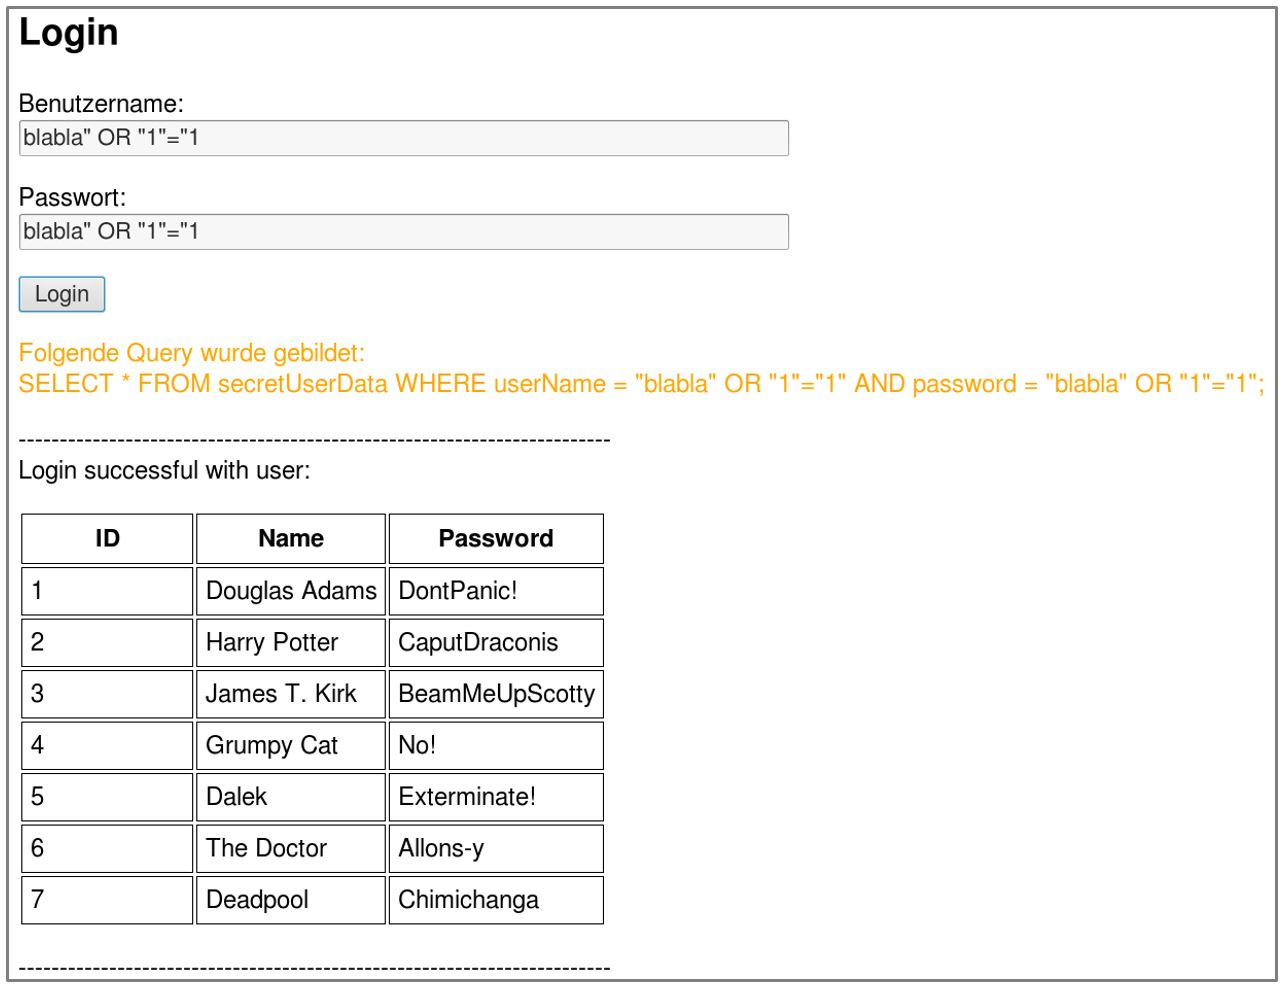
\includegraphics[width=\textwidth]{images/SQL_Injection/select_injection.jpg}
	\caption{Login mit SELECT-Injection}
	\label{fig:select_injection}
\end{figure}

Nun wurden alle Tupel, die in der Tabelle \enquote{secretUserData} enthalten sind ausgegeben. Möglich ist das durch das Anhängen von z.B. \colorbox{altgray}{\lstinline|OR "1"="1|} an eine beliebige Eingabe. Hierdurch werden die Abfragen der WHERE-Klausel grundsätzlich zu TRUE ausgewertet. Am obigen Beispiel erläutert bedeutet dies:
\begin{figure}[H]
	\centering
	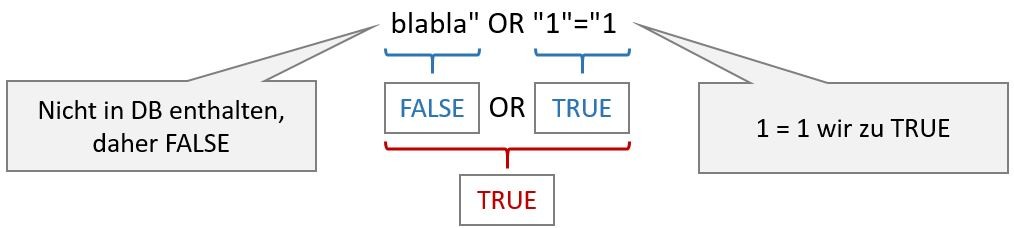
\includegraphics[width=\textwidth]{images/SQL_Injection/or1is1.jpg}
	\caption{Auswertung von OR "1"="1}
	\label{fig:or1is1}
\end{figure}
Sobald alle Ausdrücke innerhalb der WHERE-Klausel zu TRUE evaluiert wurden, wird die gesamte Datenbanktabelle ausgegeben. Hängt man den Zusatz lediglich an das Eingabefeld für das Passwort an, erhält man den Datensatz für den eingegebenen Benutzer. Dieses Szenario ist z.B. typisch, wenn man bereits einen möglichen Benutzernamen für die Applikation kennt, aber dessen Passwort unbekannt ist.

\subsection{SQL-Injection zum Einfügen von Daten}
Im zweiten Teil des Tutorials wird mittels einer SQL-Injection ein zusätzlicher Datensatz in die Tabelle eingefügt. Die Beispiel-Applikation ist äquivalent zu der aus dem ersten Tutorial. Dieses mal hängen wir an einen \colorbox{altgray}{\lstinline|beliebigen Benutzernamen|} folgendes INSERT-Statement inkl. Kommentar an: \shorthandoff{"}\colorbox{altgray}{\lstinline|"; INSERT INTO secretUserData VALUES(1234, "Hackerman", "fsociety"); --|}\shorthandon{"} . Im Eingabefeld für das Passwort können ebenfalls beliebige Zeichen eingegeben werden.
Durch diese Injection werden dem DBS prinzipiell drei Befehle übergeben:

\begin{figure}[H]
	\centering
	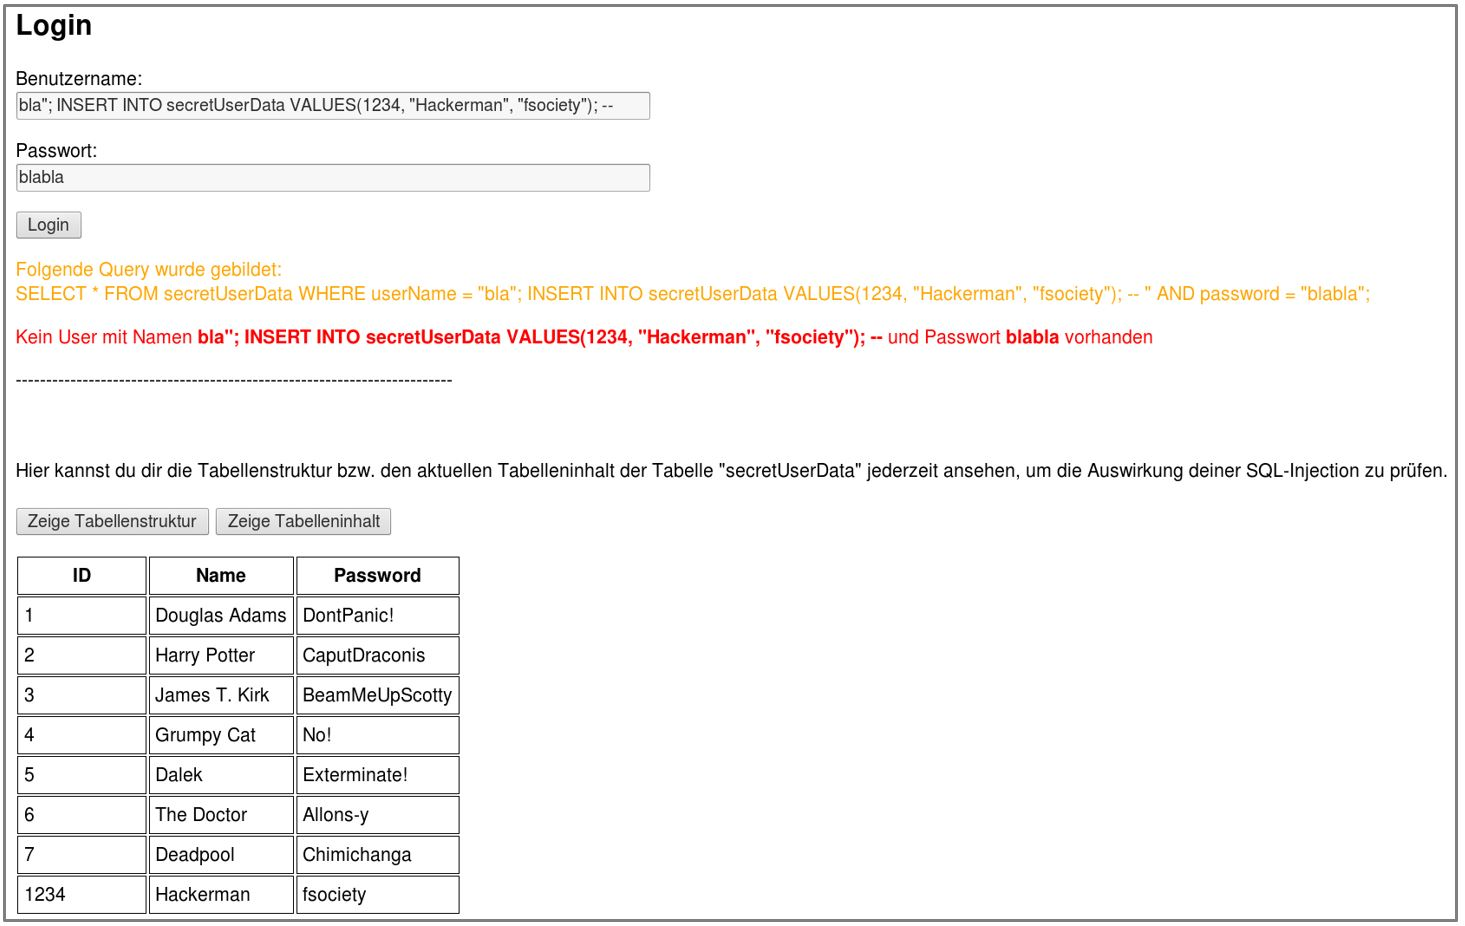
\includegraphics[width=\textwidth]{images/SQL_Injection/insert_injection.jpg}
	\caption{Login mit INSERT-Injection}
	\label{fig:insert_injection}
\end{figure}

\begin{itemize}
	\item Das ursprüngliche SELECT-Statement bis zur Eingabe eines Benutzers:  \colorbox{altgray}{\lstinline|SELECT * FROM secretUserData WHERE username = "<übergebener Benutzername>";|}
	\item Das angehängte INSERT-Statement:\\ \shorthandoff{"}\colorbox{altgray}{\lstinline|INSERT INTO secretUserData VALUES(1234, "Hackerman", "fsociety");|}\shorthandon{"}
	\item Ein Kommentar, der in SQL mit zwei Bindestrichen eingeleitet wird: \colorbox{altgray}{\lstinline|--|}. Hierdurch wird der SQL-Code, der noch zum ursprünglichen SELECT-Statement gehört, als Kommentar vom SQL-Interpreter ignoriert. Im Beispiel betrifft das: \shorthandoff{"}\colorbox{altgray}{\lstinline|" AND password = "<übergebenes Passwort>";|}\shorthandon{"}
\end{itemize}

Sieht man sich nach der Ausführung des Statements die Inhalte der Tabelle an, ist zu sehen, dass sich ein neuer Datensatz mit der User-ID 1234, dem Usernamen \enquote{Hackerman} und dem Passwort \enquote{fsociety} enthält. Nutzt man für die Injection zusätzlich einen existierenden Benutzernamen statt der Eingabe \enquote{bla}, wird man gleichzeitig bei der Applikation angemeldet.

\subsection{SQL-Injection zum Löschen von Tabellen}
Im dritten Teil des Tutorials wird mittels einer SQL-Injection die komplette Tabelle gelöscht (DROP).
 
Bitte beachte, dass du die Datenbank erst im Hauptmenü des Konsolen-Skripts im Unterpunkt \enquote{5. Datenbank zurück setzen} wieder initialisieren musst, wenn du nach dem DROP weiterarbeiten möchtest! 
 
Nun hängen wir an einen \colorbox{altgray}{\lstinline|beliebigen Benutzernamen|} folgendes Statement inkl. Kommentar an: \shorthandoff{"}\colorbox{altgray}{\lstinline|"; DROP TABLE secretUserData; --|}\shorthandon{"} . Im Eingabefeld für das Passwort können ebenfalls beliebige Zeichen eingegeben werden.
 
\begin{figure}[H]
	\centering
	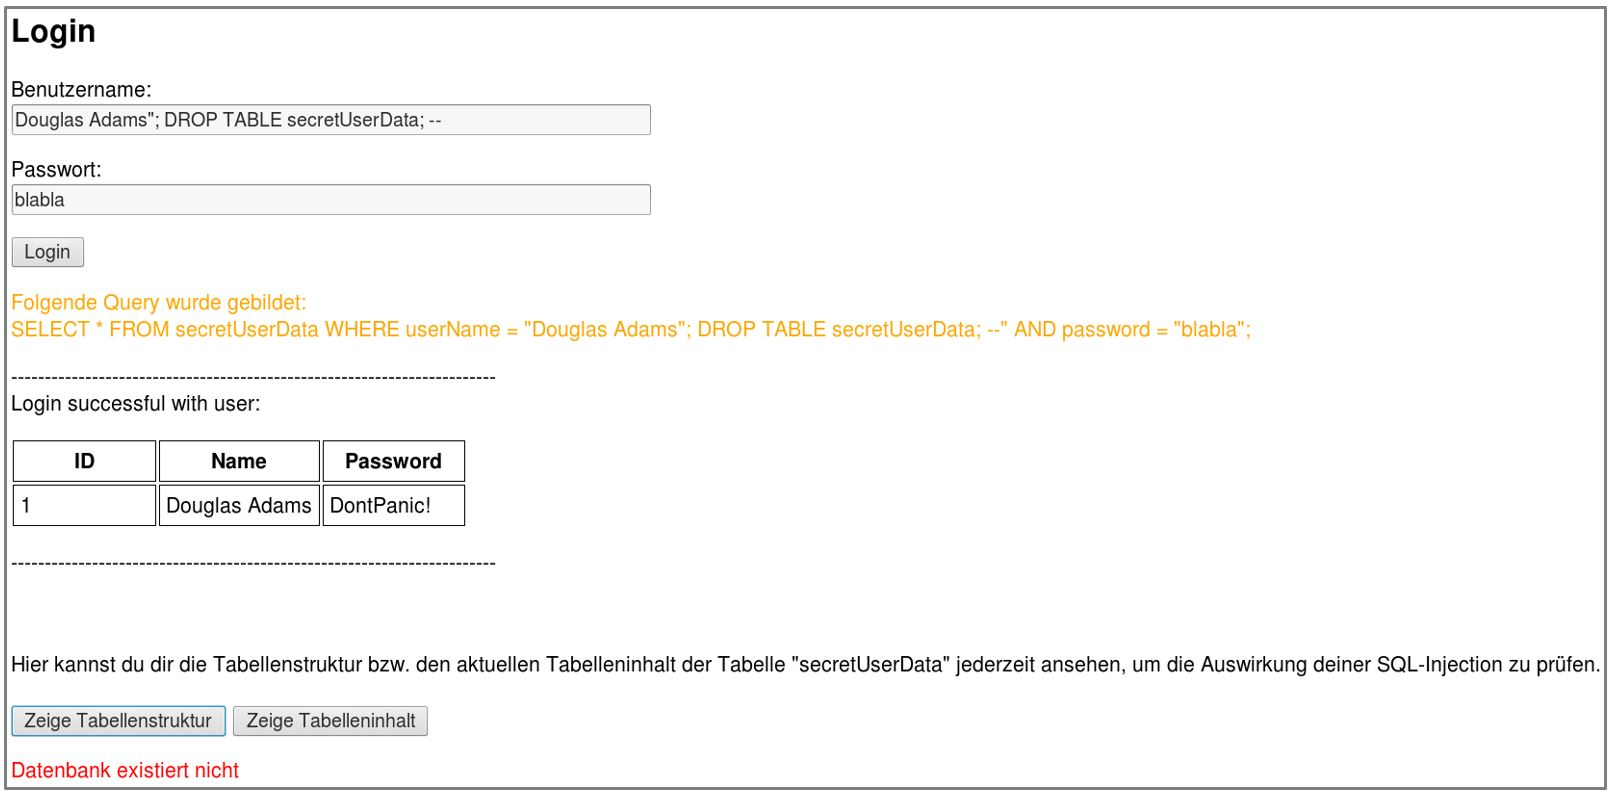
\includegraphics[width=\textwidth]{images/SQL_Injection/drop_injection.jpg}
	\caption{Login mit DROP-Injection}
	\label{fig:drop_injection}
\end{figure}

Die Ausführung der drei Statements (SELECT, DROP, Kommentar) ist äquivalent zum vorherigen Beispiel.

\subsection{SQL-Injection zum Modifizieren von Tabellen}
Das vierte Tutorial befasst sich mit modifizierenden SQL-Queries, die den Inhalt einer bestehenden Datenbanktabelle verändern. Technisch wird dies mit dem Update-Statement realisiert (siehe Listing \ref{lstlisting:SQL-UPDATE-Statement}).

\begin{lstlisting}[caption=SQL-UPDATE-Statement\label{lstlisting:SQL-UPDATE-Statement}]{Name}
$query = '
	UPDATE table_name
	SET column1 = value1, column2 = value2, ...
	WHERE condition; 
';
\end{lstlisting}
In Bezug auf das Tutorial umfasst die Datenbank eine Tabelle \colorbox{altgray}{\lstinline|sqlRanking|}, die eine virtuelle Rangliste entspricht (siehe Abbildung \ref{fig:sql-modify-ranking}). Diese besitzt die Spalten Username und Punkte. Zudem wird während der Initialisierung der Webseite die Rangliste auf Basis der Punktzahl absteigend sortiert.

\begin{figure}[H]
	\centering
	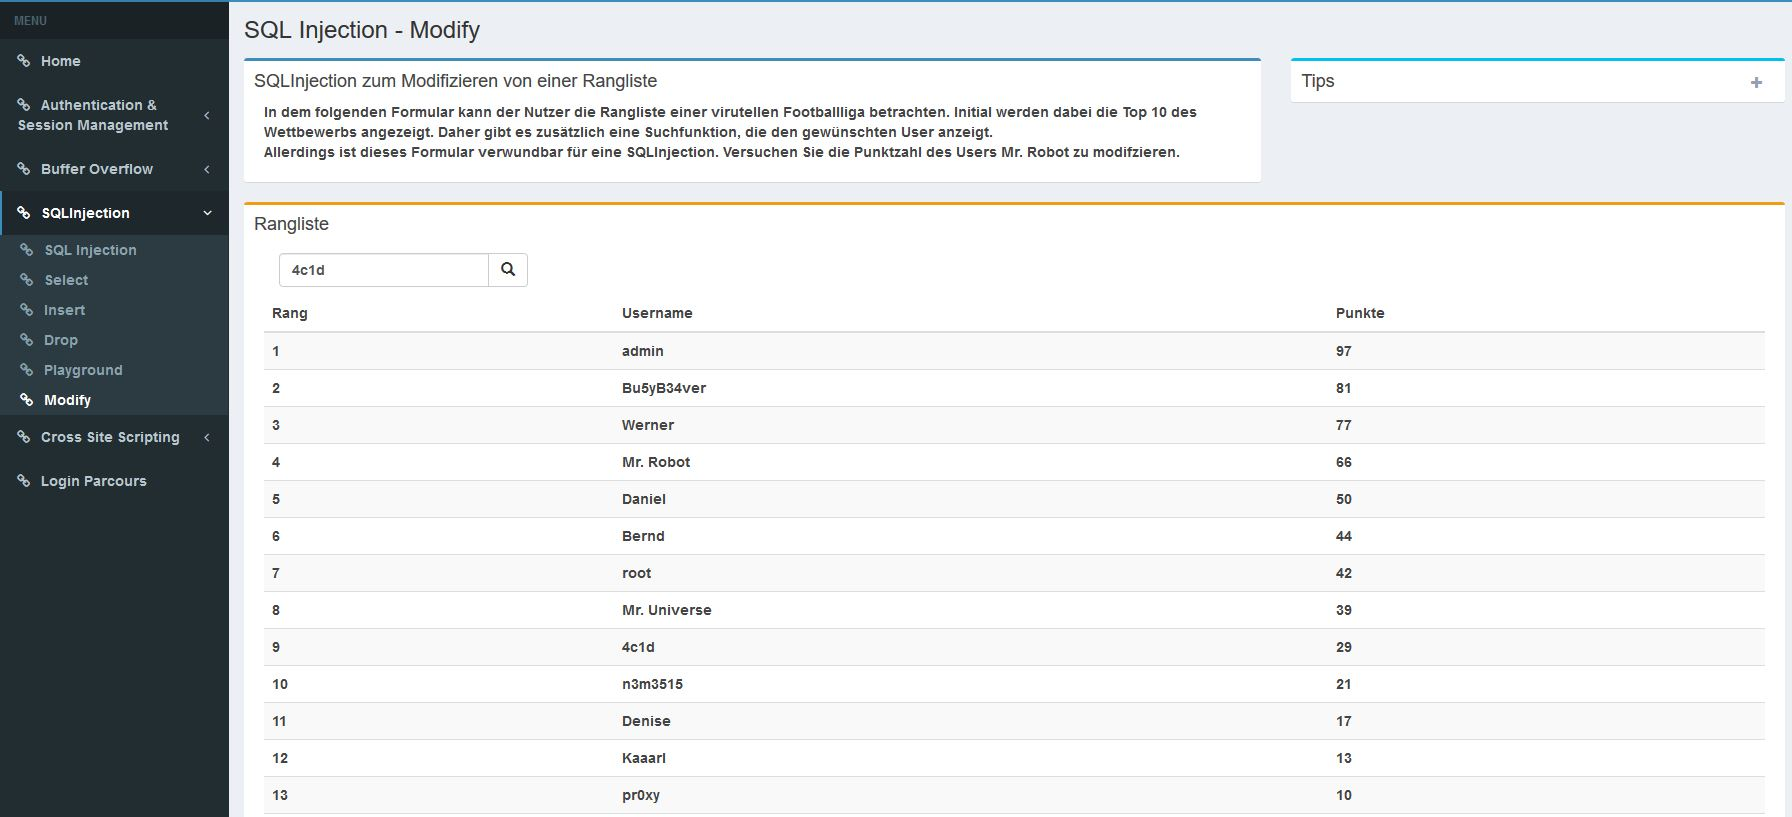
\includegraphics[width=\textwidth]{images/SQL_Injection/sql_modify.jpg}
	\caption{Rangliste mit Suchfunktion}
	\label{fig:sql-modify-ranking}
\end{figure}

Als Anwendungsszenario ist es hierbei möglich, die Rangliste mit einer Suchfunktion nach bestimmten Usernamen zu filtern. Abbildung \ref{fig:sql-modify-ranking-searched} zeigt wie der Anwender mit Hilfe des Input-Feldes nach einem gewünschten User sucht. Die Kommunikation mit der Datenbank basiert hierbei auf einem einfachen SELECT-Query.

\begin{figure}[H]
	\centering
	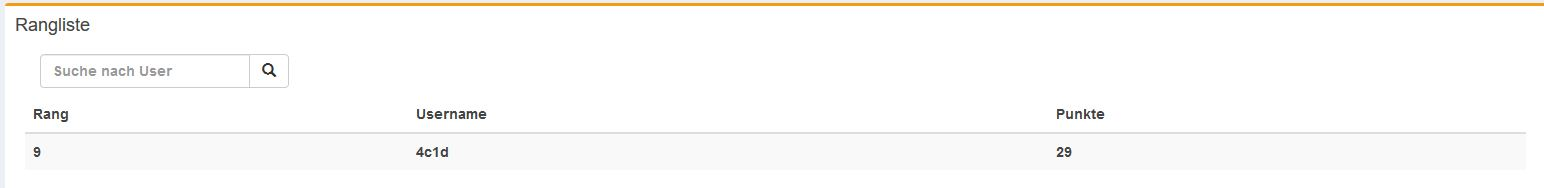
\includegraphics[width=\textwidth]{images/SQL_Injection/sql_modify_searched.jpg}
	\caption{Rangliste mit gesuchtem User}
	\label{fig:sql-modify-ranking-searched}
\end{figure}

An dieser Stelle gilt es hervorzuheben, dass die SQL-Abfrage nicht absichert ist und somit eine Sicherheitslücke entsteht. Im Folgenden ist das Ziel des Tutorials die Punkteanzahl eines Users zu modifizieren. 

Um die Aufgabe zu lösen, muss der Anwender in das Input-Feld ein SQL-Statement einfügen, das bspw. \\ \colorbox{altgray}{\lstinline|';  UPDATE sqlInjectionRanking SET punkte = 999 WHERE username = 'Mr. Robot|} entspricht. Wichtig ist das die erste SELECT-Abfrage gültig ist. Abbildung \ref{fig:sql-modify-ranking-solved} zeigt wie die Lösung des Tutorials aussehen kann. 

\begin{figure}[H]
	\centering
	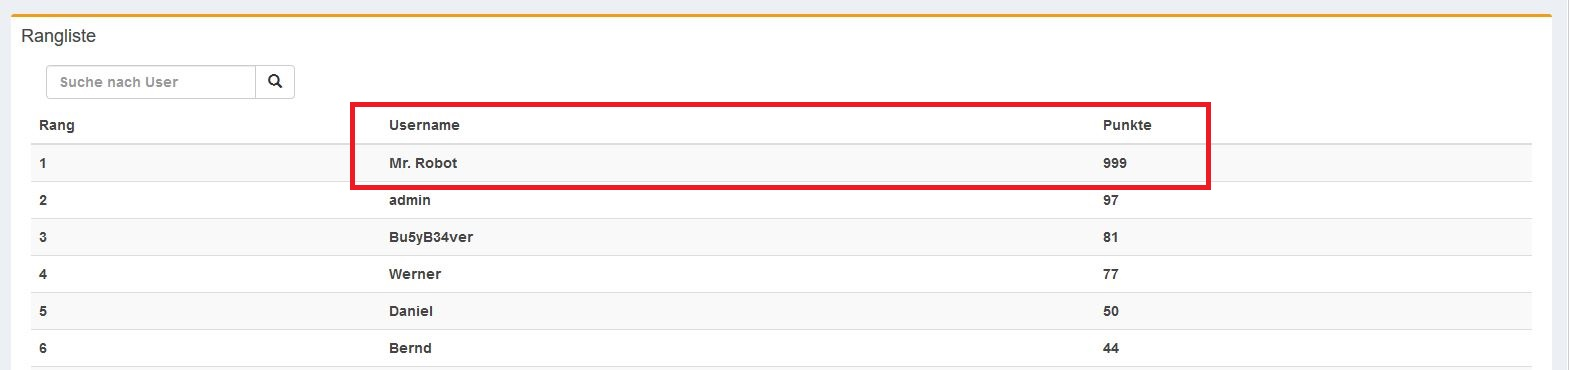
\includegraphics[width=\textwidth]{images/SQL_Injection/sql_modify_solved.jpg}
	\caption{Rangliste mit gesuchtem User}
	\label{fig:sql-modify-ranking-solved}
\end{figure}

Um das Tutorial zu vereinfachen, bekommt der Anwender je nach Wissensstand Tipps an die Hand, die ihn zur Lösung der Aufgabe hinführen sollen. 


\subsection{Die SQL-Injection-Spielwiese}
Im letzten Tutorial der SQL-Injection in der Broken-Web-Anwendung findest du die SQL-Injection-Spielwiese. Innerhalb dieser Spielwiese kannst du beliebige SQL-Injections ausprobieren.

\begin{figure}[H]
	\centering
	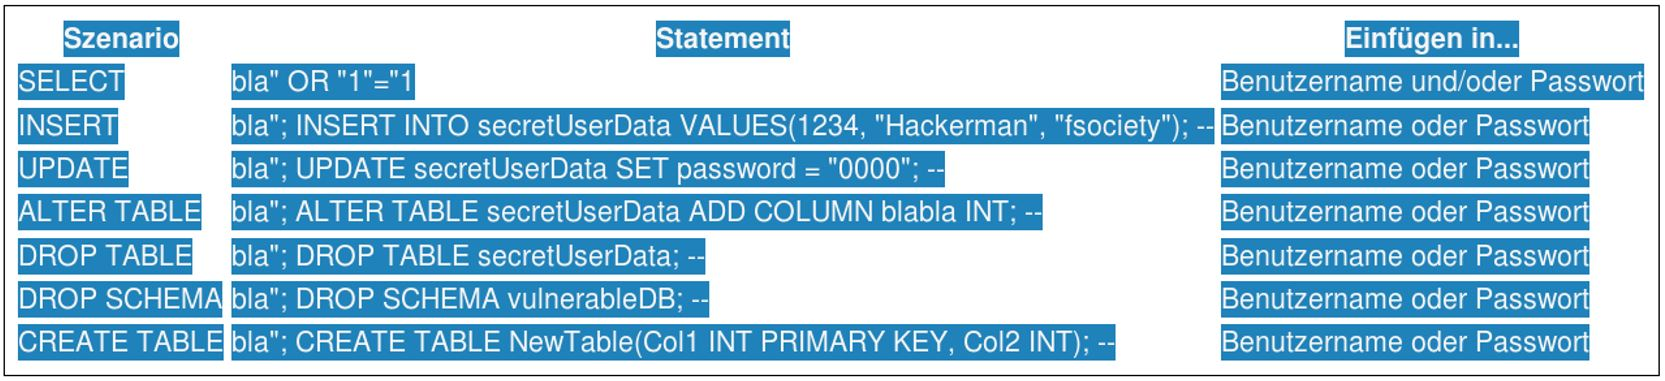
\includegraphics[width=\textwidth]{images/SQL_Injection/various_injections.jpg}
	\caption{Verschiedene SQL-Injections zum Ausprobieren}
	\label{fig:various_injections}
\end{figure}

Als Hinweis sind die Statements der vorhergegangenen Beispiele und einige Weitere im nachfolgenden Fenster hinterlegt. Um sie zu sehen musst du lediglich den Inhalt des Fensters mit der Maus markieren. Bitte beachte, dass du die Datenbank im Hauptmenü des Konsolen-Skripts im Unterpunkt \enquote{5. Datenbank zurück setzen} wieder initialisieren musst, wenn du nach einer Datenstruktur verändernden SQL-Injection weiter arbeiten willst. Dazu musst du die Anwendung nicht schließen. Deine Änderungen am Inhalt oder an der Struktur der Datenbank kannst du mit der Anzeige der Tabellenstruktur bzw. dem Inhalt jederzeit prüfen.\\

Neben den hier aufgelisteten gibt es noch eine Vielzahl weiterer SQL-Injections. Nicht alle werden in diesem Beispiel funktionieren, da der Erfolg von SQL-Injections von mehreren Faktoren abängig ist:
\begin{itemize}
	\item Die Programmiersprache der Anwendung
	\item Das verwendete DBMS
	\item Die Berechtigungen, die der Datenbankbenutzer der Anwendung inne hat
\end{itemize}

\section{Gegenmaßnahmen}
Viele Programmiersprachen haben mittlerweile Mechanismen eingebaut, mittels derer SQL-Injections abgewehrt werden können. So ist es in den meisten Programmier- und Skriptsprachen nicht mehr möglich, innerhalb eines DB-Aufrufs mehrere SQL-Statements auszuführen. In einigen wenigen ist dies immer noch möglich, wie z.B. in der Skriptsprache PHP.
\subsection{Prepared Statements}
Durch sogenannte \enquote{Prepared Statements} können SQL-Injections vollständig unterbunden werden. Statt das SQL-Statement komplett auf der Applikationsseite zusammenzustellen, wird das Statement auf zwei Mal an das DBS gesendet. Im ersten Aufruf wird das vorbereitete Statement ohne die Nutzereingaben an das DBS übermittelt. Hierdurch wird dem DBS die Struktur des Statements im Vorfeld angekündigt. Nachfolgend ist das Prepared Statement eines SELECT-Statements zu sehen:
\begin{lstlisting}[caption=Prepared Statement]{Name}
prepare("SELECT * FROM secretUserData where userName = ?");
\end{lstlisting}

Die vom Nutzer eingegebenen Parameter werden erst im Anschluss an das DBS übermittelt:
\begin{lstlisting}[caption=Übergabe der Parameter]{Name}
execute($_GET['name']);
\end{lstlisting}
Dort werden sie in das bereits angekündigte Statement eingefügt und ausgeführt. Übergebene Parameter, auch wenn ihnen SQL-Code hinzugefügt wurde, werden ausschließlich als Textinput interpretiert. 
\subsection{Escapen von Eingaben}
Eine weitere Möglichkeit die Datenbank vor unberechtigtem Zugriff und Manipulationen zu schützen ist das Escapen aller Nutzereingaben.
Das grundlegende Problem bei SQL-Injections ist die Interpretation von Texteingaben als ausführbare Anweisungen für das DBMS. Durch das Escapen der Eingaben werden Metazeichen wie Anführungszeichen maskiert und somit vom SQL-Interpreter nicht beachtet. Nachfolgend ist das Escapen von Strings in PHP dargestellt:
\begin{lstlisting}[caption=Escapen von Strings in PHP]{Name}
mysql_real_escape_string("some String");
\end{lstlisting}
